%%%%%%%%%%%%%%%%%%%%%%%%%%%%%%%%%%%%%%%%%%%%%%%%%%%%%%%%%%%%%%%%%%%%%%%
% Preamble
%%%%%%%%%%%%%%%%%%%%%%%%%%%%%%%%%%%%%%%%%%%%%%%%%%%%%%%%%%%%%%%%%%%%%%%%
\documentclass[11pt]{article}
%
% Packages and other includes
% Pagination
\usepackage[letterpaper, margin=1.25in]{geometry}
%
% Graphics, floats, tables
\usepackage{graphicx, color, float, array}
%
% Hyperlinks
\usepackage{hyperref}
%
% AMS packages for equations, math symbols
\usepackage{amsmath, amssymb, braket}
%
% Bibliography
\usepackage[style=numeric,sorting=none]{biblatex}
\addbibresource{references.bib}
%
% Revision (see Makefile)
\newcommand{\Revision}{977be36}

%
% Definitions and settings
% Paragraph indent and spacing
\setlength{\parskip}{0.4\baselineskip}
\setlength{\parindent}{0in}
%
% Math mode version of "r" column type (requires array package)
\newcolumntype{R}{>{$}r<{$}}
%
% Title, authors, date
\title{\textbf{Uncovering the Chirality of Triazasumanene}}
\author{Brian Nguyen}
\date{Chem 150L Winter 2018 \\ \today, Revision \Revision}
%
%
%%%%%%%%%%%%%%%%%%%%%%%%%%%%%%%%%%%%%%%%%%%%%%%%%%%%%%%%%%%%%%%%%%%%%%%%
% Main document
%%%%%%%%%%%%%%%%%%%%%%%%%%%%%%%%%%%%%%%%%%%%%%%%%%%%%%%%%%%%%%%%%%%%%%%%
%
\begin{document}

\maketitle

\begin{abstract}
  \noindent Few heteroatom-doped buckybowls have been synthesized and
  thoroughly studied for rational design of the next generations of buckybowls.
  This may be attributed to the difficulty of synthesizing buckybowls and
  understanding the stabilities of these structures. The chirality of
  triazasumanene is investigated to understand the overall energetics and
  to provide an avenue for the possibility of combining computational and
  experimental work to synthesize the next generation of heteroatom-doped
  sumanene. A theoretical study was launched performing geometry ground state
  optimization, transition state optimization, and circular dichromism
  spectrum.
\end{abstract}

\section{Introduction}

Miniaturization of novel devices and machines on a molecular level
has been one of the main goals in electronics\cite{Vincenzo}. The decreasing
device size may lead to greater power and funcationality residing on
a chip. For instance, polycyclic aromatic carbons with curved $\pi$-conjugated
structures, such as fullerenes, carbon nanotubes, and buckybowls
are appealing materials due to their low density, structural stability,
and extended-delocalized $\pi$ networks that support mobile charge
carriers\cite{Laura}. However, few heteroatom-doped buckybowls
have been synthesized and reported. The most recent successful
synthesis of triazasumanene is an isoelectronic heteroanalogue
of sumanene from Tan et. al.\cite{doi:10.1246/bcsj.20170384}

First principle calculations may provide insights on the electronic
structures of these sumanene derivatives and improve upon the
current state-of-the-art. In this report, we provide a theoretical
investigation of the triazasumanene by computing the optimized
ground state and transition state structures with the corresponding
electronic circular dichroism (ECD) that may lead to further
joint computational and experimental studies.

\section{Methods}

\subsection{Statement of the Models}

A racemic mixture is a 50:50 mixture of two enantiomers. In the synthesis
of triazasumanene, two absolute stereochemical configurations coexisist
which are designated as clockwise (C) and counterclockwise (A) as shown
in Fig \ref{fig:stereo}. The configuration is based on the heteroatoms
having the lowest possible number.

\begin{figure}[htbp]
  \center
  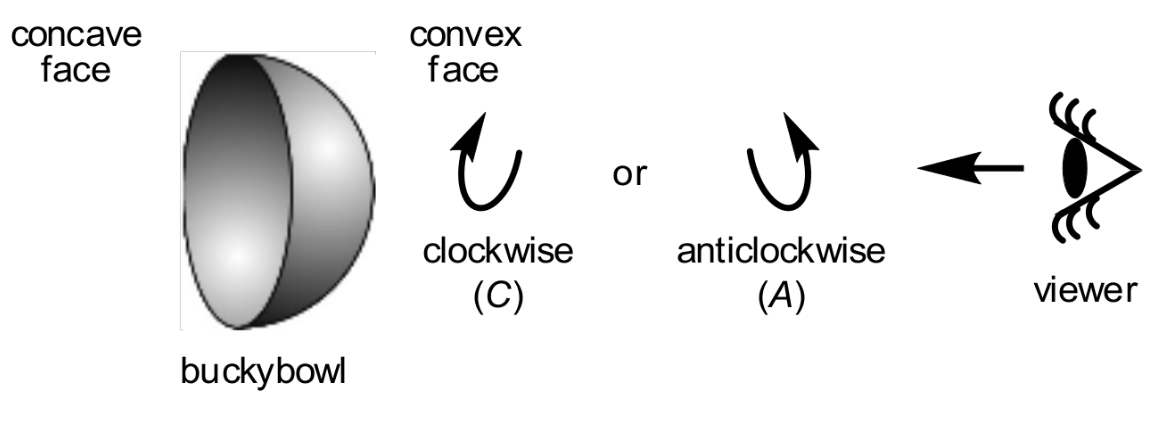
\includegraphics[scale=0.25]{buck.png}
  \caption{An illustration demonstrating the nomenclature of buckybowl
    enantiomers.}
  \label{fig:stereo}
\end{figure}

To resolve the racemic triazasumanene, one method is to use electronic
circular dichroism (ECD) spectroscopy coupled with electronic structure
calculations.

\subsection{Computational Details}

Within the TURBOMOLE v7.2 suite\cite{TURBOMOLE}, the aoforce and escf module are
used to compute the vibrational frequencies and generate the ECD spectrum. The
triazasumanene structure was constructed on avogadro v1.2\cite{Hanwell2012}
and minimized with universal force field (UFF). This initial structure was fairly
planar and this initial guess was used to optimize with TPSS\cite{PhysRevLett.91.146401}
using def2-SV(P) basis and D3 dispersion correction\cite{doi:10.1002/jcc.21759}.
A total of three transition states were optimized from the structure built in avogadro.
Two of the transition states were constrained with C$_{3h}$ symmetry while the third
was constrained with C$_3$ symmetry.

\section{Results}

\begin{figure}[H]
  \centering
  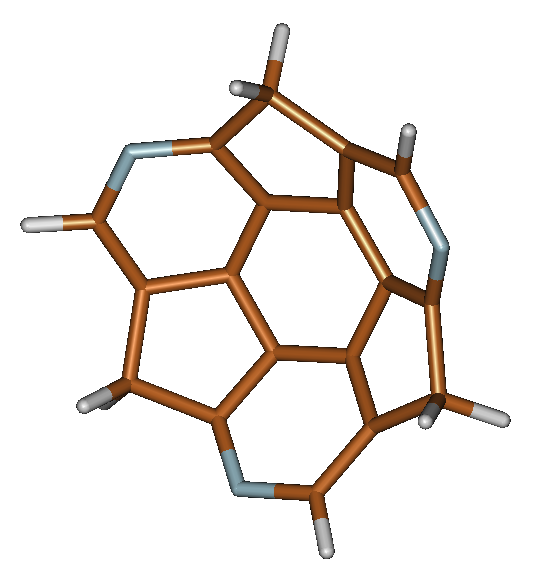
\includegraphics[scale=0.25]{opt.png}
  \caption{The optimized ground state configuration of (C)-triazsumanene using TPSS
    functional with def2-SV(P) basis set.}
  \label{fig:optimized}
\end{figure}

Triazsumanene was successfully optimized falling toward the (A) configuration verfied
through harmonic vibrational analysis and revealing a C$_3$ point group symmetry as
seen in Fig \ref{fig:optimized}. Following the ground state optimization, a transition
state search was performed and a total of three transition states were found. The
starting geometry was generated from avogadro v1.2\cite{Hanwell2012} with a fairly
planar structure. The C$_{3h}$ constrained optimization lead to a structure that
breaks C-C bonds while the C$_3$ constraint maintained the planarity of the ring
structures (Fig \ref{fig:trans}). 

\begin{figure}[H]
  \center
  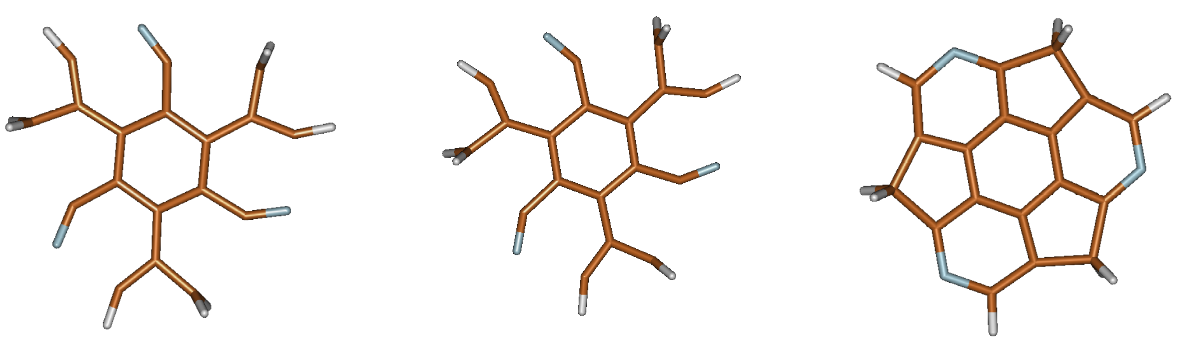
\includegraphics[scale=0.25]{transition_states.png}
  \caption{Symmetry constrained optimized structures of three transition states where
    the C$_{3h}$ symmetry (left and middle) and C$_3$ symmetry (right) were applied. The
    structures are labeled from left to right as transition states 1, 2, and 3.}
  \label{fig:trans}
\end{figure}

A closer look at the free energies of the transition states reveal that the
optimized transition state constrained with C$_3$ symmetry has a closer
racemization energy to the experimental result of 38.2 kcal/mol at
476K\cite{doi:10.1246/bcsj.20170384}. This may be attributed to the broken C-C
bonds seen in the C$_{3h}$ symmetry constrained optimization (Tab \ref{energy}).
In addition, the harmonic vibrational analysis of the transition state structures
revealed that the C$_3$ symmetry constrained transition state is verfied to be
a transition state due to having only 1 imaginary frequency.

\begin{table}[H]
  \caption{The transition state free energies computed with TPSS-D3 and def2-SV(P)
    basis set. Transition states 1 and 2 were constrained with C$_{3h}$ symmetry while
    transition state was constrained with C$_3$ symmetry. Racemization barrier is
    computed by taking the difference in free energy between the ground state and
    transition state. The total free energy of the ground state is -5.3649E5 kcal/mol.}
  \begin{tabular}{c|cc}
    Transition State & Total Free Energy (kcal/mol) & Racemization Barrier (kcal/mol) \\
    \hline\hline
    1 & -5.3621E5 & 279.25\\
    2 & -5.3623E5 & 262.55\\
    3 & -5.3645E5 & 40.85\\
  \end{tabular}
  \label{tab:energy}
\end{table}

Lastly, the CD spectrums of both absolute configurations (A)- and (C)-triazasumanene
were computed and the spectrums reveal unique rotary strength at different wavelengths
(Fig \ref{fig:cdspec} and \ref{fig:opt2cd}).

\begin{figure}[H]
  \center
  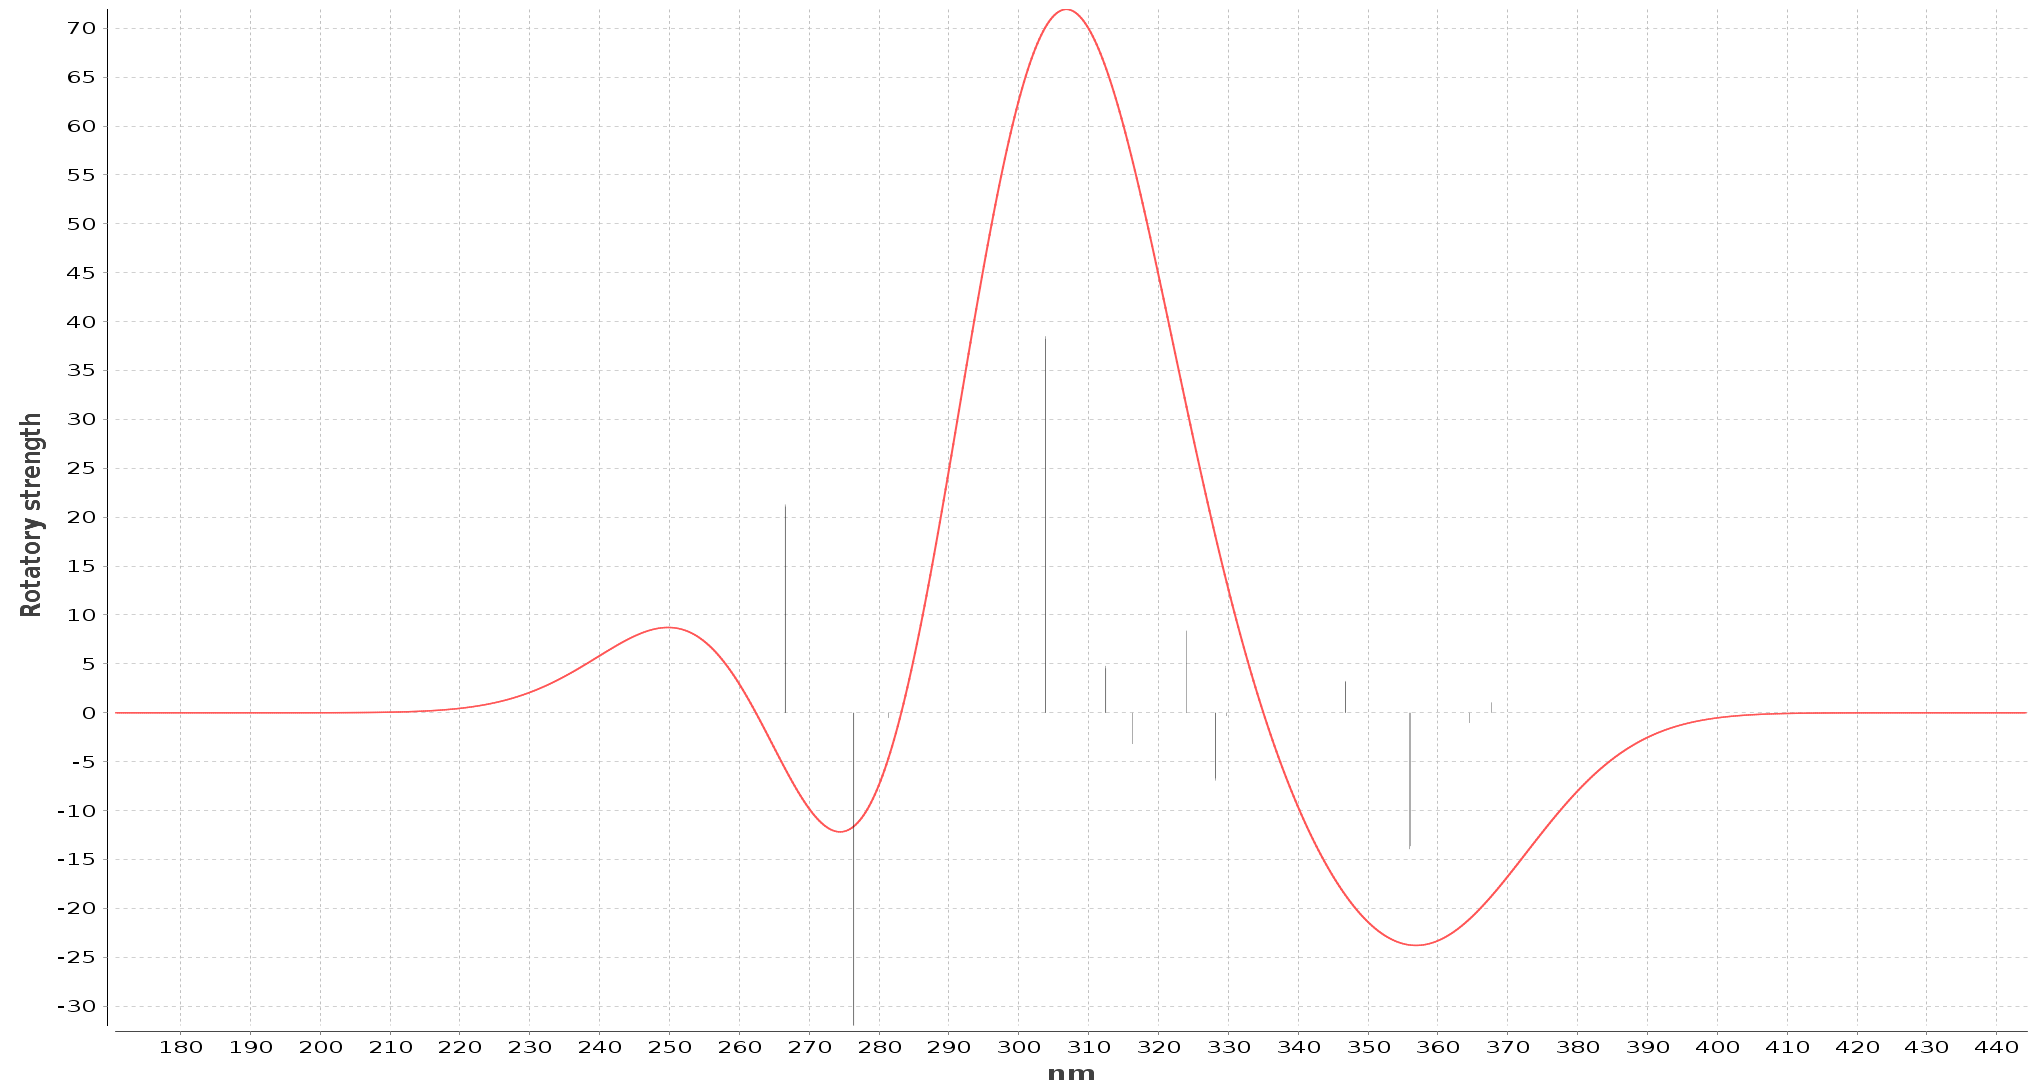
\includegraphics[scale=0.2]{cd_spec.png}
  \caption{This is a computed CD spectrum of the ground state (A)-triazasumanene for the
    first 20 dipole allowed excitations and broadened rotary strengths with Guassians
    using 0.16 eV linewidth.}
  \label{fig:cdspec}
\end{figure}

\begin{figure}[H]
  \center
  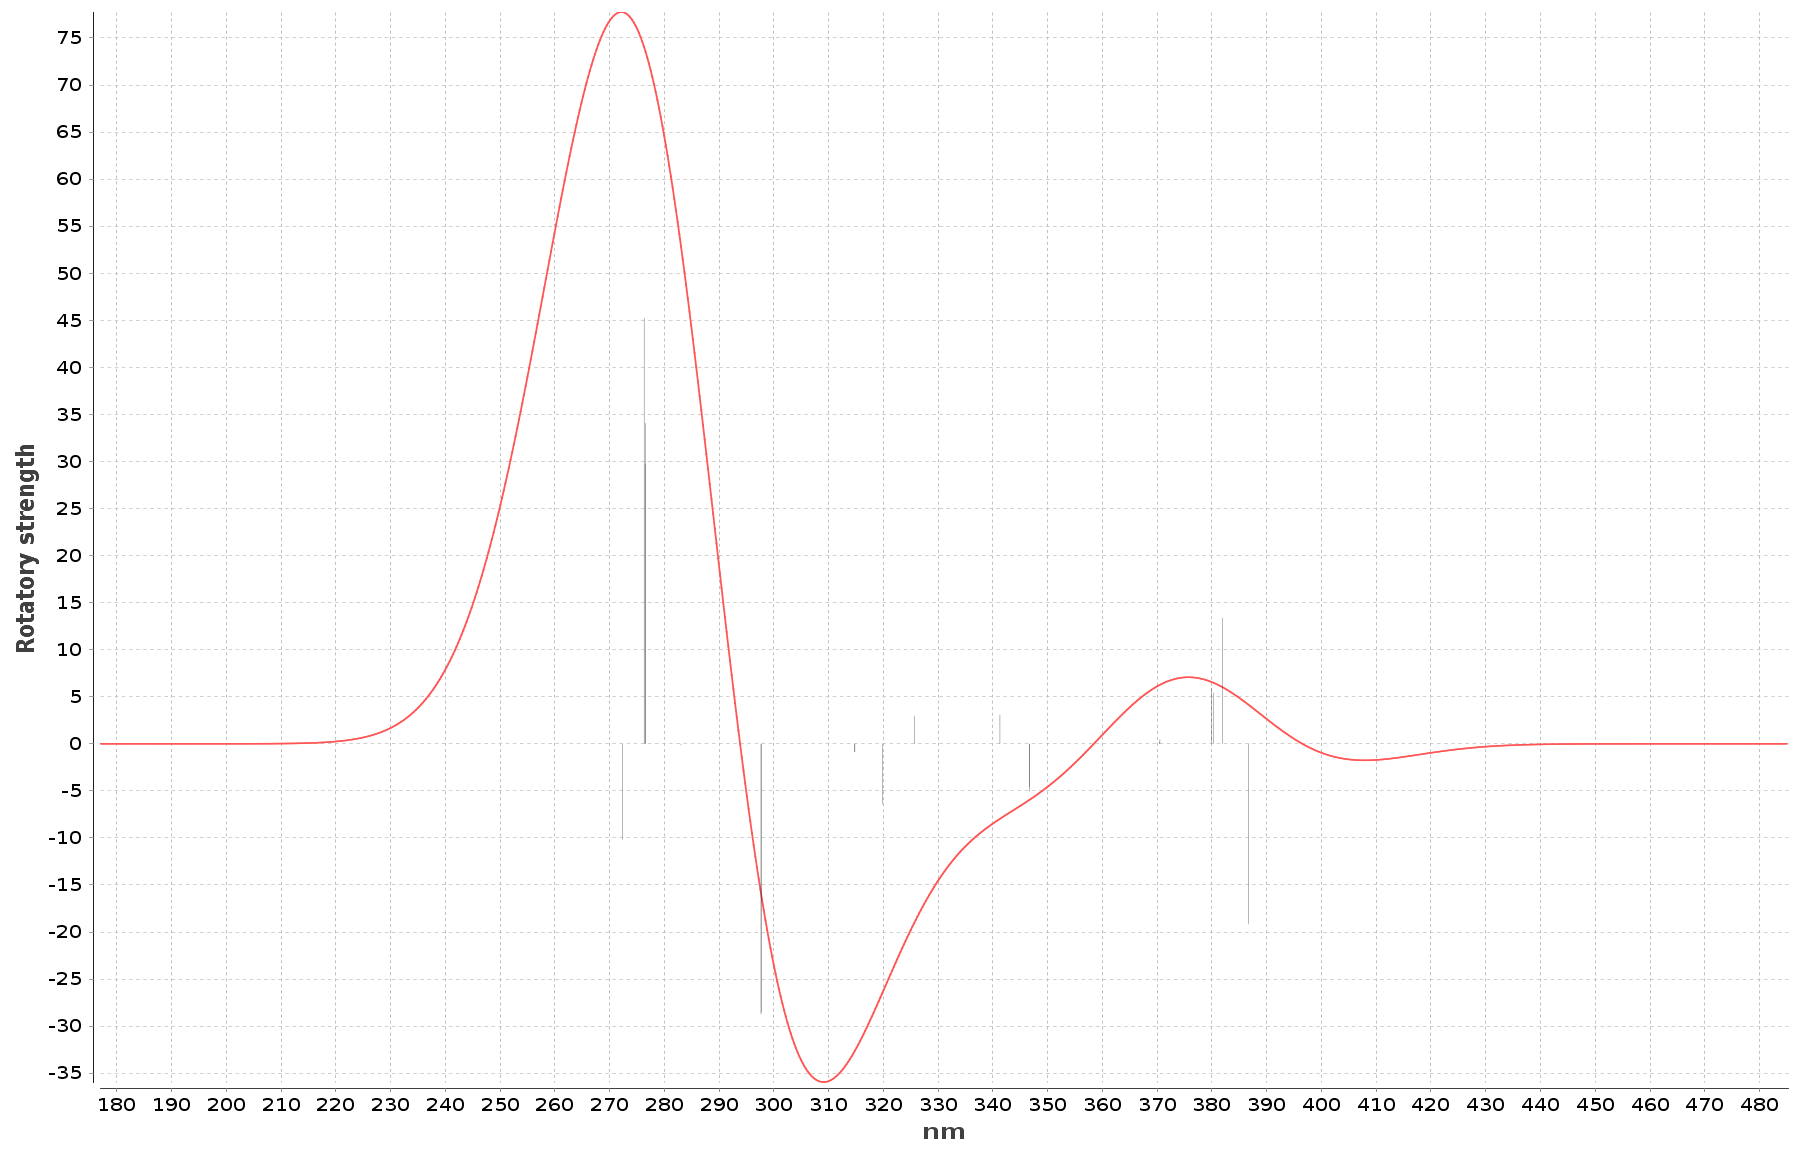
\includegraphics[scale=0.2]{opt2_cd.png}
  \caption{The CD spectrum of (C)-triazasumanene for the first 20 dipole allowed excitations
    and broadened rotary strengths with Guassians using 0.16 eV linewidth.}
  \label{fig:opt2cd}
\end{figure}

\section{Conclusions}

In summary, the elucidation of the chirality of triazasumanene can be achieved
through computation as seen by the free energy calculations and computed CD
spectrum of both absolute configurations (A) and (C). Three transition states
were found and it was discovered that only the C$_3$ symmetry constrained
transition state was valid. Moreover, the computed CD spectrum was fairly close
to experimental CD spectra\cite{doi:10.1246/bcsj.20170384} for the excitation at
around 272 nm. However, the lower excitations did not align with the experimental
CD spectra\cite{doi:10.1246/bcsj.20170384}. The work presented provides a baseline
for future improvement to computational studies of triazasumanene. 

\printbibliography

\end{document}
